\documentclass{beamer}
\usepackage[ngerman]{babel}			%Deutsche Umlaute und Umbrüche
\usepackage[utf8]{inputenc}			%utf8 Kodierung
\usepackage{amsmath, amsfonts, amssymb} %Mathepackete schaden nie
\usetheme{Dresden}
\usecolortheme{beaver}
\usefonttheme{professionalfonts}
\title[WWWEKA]{World Wide WEKA}
\subtitle{Requirement Document}
\author[C. Heckmann\and C. Stricker\and D. Klopp\and M. Vieth]{Christian Heckmann\and Christian Stricker\and David Klopp\and Markus Vieth}
\date[01.01.1111]{01. Januar 1111}
\subject{Software engineering}
%Link zum Beamer-Userguid: ftp://ftp.dante.de/tex-archive/macros/latex/contrib/beamer/doc/beameruserguide.pdf
\begin{document}
	
	\frame{
		\titlepage
	}
	\setbeamertemplate{footline}[frame number]
	
	\frame[label=IV]{
		\frametitle{Inhaltsverzeichnis}
		\tableofcontents
		[pausesections]
	}
	
	\section[UR 1]{User Requirement Beispiel 1}
	\subsection[Statement]{Statement}
	\begin{frame}{Statement}{Browser}
		"Das System soll über alle gängigen Browser nutzbar sein (Desktop und Mobile): Firefox, Chrome, Opera, Internet Explorer."
	\end{frame}
	
	\subsection[Resultierende Fragen]{Resultierende Fragen}
	\begin{frame}[<+->][t]{Resultierende Fragen}
		\begin{itemize}		
			\item Welche Browser werden aktuell verwendet?
			\item Welche Browserversionen werden häufig eingesetzt?
			\item Werden die benötigten Funktionen unterstützt (HTML5, JavaScript)?
			\item Werden alle Plattformen abgedeckt (Smart Device, Desktop)?
		\end{itemize}
	\end{frame}
	
	\subsection[Browser]{Browser}
	\begin{frame}[t]{Browserversionen}
		\begin{figure}
\centering
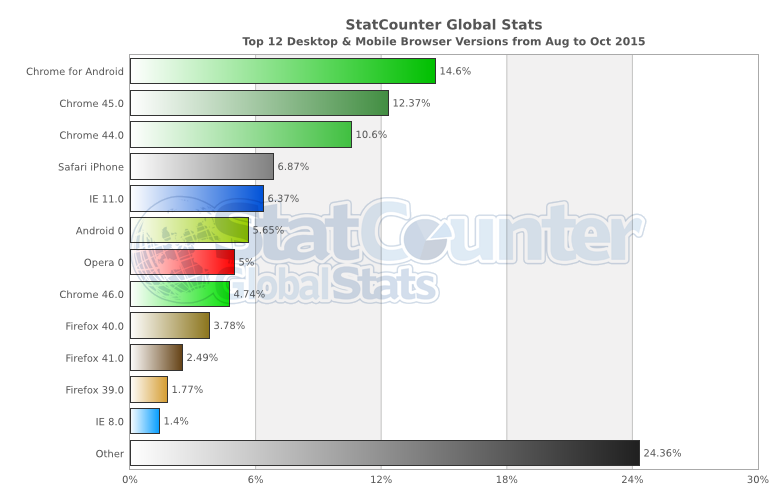
\includegraphics[width=1\linewidth]{../../../Downloads/StatCounter-browser_version-ww-monthly-201508-201510-bar}
\label{fig:StatCounter-browser_version-ww-monthly-201508-201510-bar}
\end{figure}

	\end{frame}
	\begin{frame}[t]{Browserversionen}
		\begin{columns}
				\column{.5\textwidth}
				\begin{description}	
				\item<1->[Google Chrome] 65,9\%
				\begin{description}
					\item<1->[4.7] 1,2\%
					\item<1->[4.6] 0,6\%
					\item<1->[4.5] 72,5\%
					\item<1->[4.4] 15,9\%
					\item<1->[4.3] 3\%
					\item<1->[4.2] 0,8\%
				\end{description}
			\end{description}
				\column{0.5\textwidth}
				\begin{description}
				\item<2->[Firefox] 20,6\%
					\begin{description}
						\item<2->[FF 42] 1\%
						\item<2->[FF 41] 9,2\%
						\item<2->[FF 40] 64,1\%
						\item<2->[FF 39] 5,3\%
						\item<2->[FF 38] 6,8\%
					\end{description}
				\end{description}
			\end{columns}
		\end{frame}
		\begin{frame}
			\begin{columns}
				\column{0.5\textwidth}
				\begin{description}	
				
				\item<1->[Internet Explorer] 6,4\%
				\begin{description}
					\item[IE 11] 65,6\%
					\item[IE 10] 14\%
					\item[IE 9] 14\%
					\item[IE 8] 7,8\%
				\end{description}
				\end{description}
				\column{0.5\textwidth}
				\begin{description}
				\item<2->[Edge] 0,8\%
				\item<3->[Android Browser] 3,24\%
				\item<3->[MobileSafari] 1,21\%
			\end{description}
			\end{columns}
	\end{frame}
	\begin{frame}[<+->][t]{Browserfunktionen}
			\begin{itemize}	
				\item Korrektheit der Daten (FR011)
				\item Algorithmus hochgeladen ? (NFR020)
				\item Verstoßen gegen bestehendes Recht (NFR031)
			\end{itemize}
			
	\end{frame}
	\begin{frame}[<+->][t]{Browser Plattformen}
			\begin{itemize}	
				\item In RDF Datenbank speichern (NFR027)
				\item Verfügbarkeit über REST-Protokoll (FR001, FR009)
				\item Dateiverwaltung (FR015)
				\item Download (FR027, 028)
			\end{itemize}
	\end{frame}
	
	\section[UR 2]{User Requirement Beispiel 2}
	\subsection[Statement]{Statement}
	\begin{frame}{Statement}{Datenupload}
			"Nutzer sollen die benötigten Datensätze, Modelle, sowie Algorithmen von einem lokalen PC auf den Server hochladen können."
	\end{frame}
	
	\subsection[Resultierende Fragen]{Resultierende Fragen}
	\begin{frame}[<+->][t]{Resultierende Fragen}
		\begin{itemize}		
			\item Welche Formate werden unterstützt?
			\item Müssen die Daten überprüft werden?
			\item Was geschieht bei zu vielen gleichzeitigen Uploads?
			\item Was geschieht mit den Daten nach dem Upload ?
			\begin{itemize}	
				\item Wer hat Zugriff auf die Daten?
				\item Wie lange bleiben die Daten erhalten?
				\item Was gilt für den Gast Nutzer?
			\end{itemize}
		\end{itemize}
	\end{frame}
	
	\subsection[Upload Prozess]{Upload Prozess}
	\begin{frame}[<+->][t]{Upload Prozess}
		\begin{itemize}		
			\item Vor dem Upload:
			\begin{itemize}	
				\item Sichere Verbindung zwischen Client und Server (NFR021)
				\item Dateiformat prüfen (FR008)
				\item Dateigröße prüfen (NFR011)
			\end{itemize}
			
			\item Nach dem Upload:
			\begin{itemize}	
				\item Korrektheit der Daten (FR011)
				\item Algorithmus hochgeladen ? (NFR020)
				\item Verstoßen gegen bestehendes Recht (NFR031)
			\end{itemize}

			\item Speicherung der Daten:
			\begin{itemize}	
				\item In RDF Datenbank speichern (NFR027)
				\item Verfügbarkeit über REST-Protokoll (FR001, FR009)
				\item Dateiverwaltung (FR015)
				\item Download (FR027, 028)
			\end{itemize}
		\end{itemize}
	\end{frame}
		
\end{document}